\chapter{Endocrinologie et homéostasie}\label{ch:b3:endocrinology}

Durant l'été 1921, deux jeunes hommes d'un laboratoire torontois
surchauffé ligaturèrent les canaux pancréatiques de chiens, attendirent
que le tissu digestif s'atrophie, broyèrent ce qui restait, et
injectèrent l'extrait à un chien rendu diabétique par l'ablation de son
pancréas. Sa glycémie tomba. En janvier un garçon de quatorze ans
mourant de diabète au Toronto General Hospital recevait l'extrait, et en
quelques semaines il mangeait, marchait et prenait du poids~; il vécut
treize ans de plus. La substance, l'\omterm{def:b3:endocrinology:glucose}{insuline}, est un peptide de
cinquante et un acides aminés sécrété dans le sang par un pour cent du
pancréas, où, à une concentration de quelques centaines de picomoles par
litre, elle dit à chaque cellule musculaire et adipeuse du corps ce
qu'il faut faire du sucre du dernier repas. Ce chapitre traite de tels
messagers~: ce qu'ils sont, comment une cellule qui n'a jamais rencontré
la glande sait ce que le message veut dire, comment les glandes sont
elles-mêmes gouvernées dans une hiérarchie de boucles de rétrocontrôle,
et comment l'ensemble tient à quelques pour cent près, une vie durant,
le glucose, le sel, le calcium et la température du sang --- et ce qui
arrive, en clinique, quand une des boucles lâche.

\section{Les hormones et leurs récepteurs}

\begin{definition}[L'hormone]\label{def:b3:endocrinology:hormone}
\index{hormone}\index{glande endocrine}\index{paracrine}\index{hormone stéroïde}\index{hormone peptidique}\index{récepteur nucléaire}
Une \emph{hormone} est une substance libérée par une cellule dans le
sang et qui agit sur des cellules lointaines porteuses de son
récepteur~; un signal \emph{paracrine} agit sur les voisines, un signal
\emph{autocrine} sur la cellule qui l'a fait, et une neurohormone est
libérée dans le sang par un neurone. Aux \emph{glandes endocrines}
classiques --- \omterm{def:b3:endocrinology:axes}{hypophyse}, thyroïde, parathyroïdes, surrénales, îlots
pancréatiques, gonades --- se sont joints le cœur (peptide
natriurétique), le rein (érythropoïétine), le tissu adipeux (leptine),
l'intestin (une douzaine de peptides) et l'os. Chimiquement les hormones
sont de trois sortes, et la chimie fixe le mécanisme. Les \emph{hormones
peptidiques et protéiques} (\omterm{def:b3:endocrinology:glucose}{insuline}, hormone de croissance, hormones
hypophysaires) sont faites sur des ribosomes, stockées en granules,
libérées par exocytose, voyagent libres dans le plasma, ne peuvent
traverser les membranes, et agissent sur des récepteurs de surface ---
couplés aux protéines~G ou à activité kinase --- par des seconds
messagers, en quelques secondes à quelques minutes~; leurs demi-vies
sont de quelques minutes. Les \emph{stéroïdes} (cortisol, \omterm{def:b3:renal-osmoregulation:controls}{aldostérone},
œstrogènes, testostérone, et le sécostéroïde qu'est la vitamine~D) sont
faits de cholestérol au fur et à mesure, non stockés, voyagent liés à
des protéines porteuses, traversent les membranes, et se lient à des
\emph{récepteurs nucléaires} qui sont eux-mêmes des facteurs de
transcription~: leurs effets prennent des heures et durent des jours.
Les \emph{amines} sont à cheval~: l'adrénaline agit à la surface en une
seconde~; les \omterm{prop:b3:endocrinology:thyroid}{hormones thyroïdiennes}, bien que dérivées d'un acide
aminé, agissent sur des récepteurs nucléaires comme les stéroïdes. Une
hormone ne signifie rien par elle-même~: la même adrénaline dilate un
vaisseau et en resserre un autre parce que leurs muscles lisses portent
des sous-types de récepteurs différents, et le même cortisol élève la
glycémie dans le foie et étouffe un \omterm{def:b3:adaptive-immunity:lymphocytes}{lymphocyte} parce que la \omterm{def:b3:chromatin-epigenetics:nucleosome}{chromatine}
des deux cellules offre à son récepteur des gènes différents.
\end{definition}

\begin{omfigure}
\begin{tikzpicture}[every node/.style={font=\scriptsize}, >=stealth]
  % peptide pathway
  \draw[thick, omDef, fill=omDef!10] (0,0) rectangle (5.2,3.4);
  \node[above] at (2.6,3.4) {hormone peptidique ou amine --- récepteur de surface};
  \draw[thick, omDef] (0,2.6) -- (5.2,2.6); \node[left, font=\tiny] at (5.2,2.75) {membrane};
  \node[circle, fill=omThm!60, inner sep=2pt, label={[font=\tiny]right:hormone}] (h1) at (1.4,3.1) {};
  \draw[thick, omDef!80!black, fill=omDef!40] (1.1,2.3) rectangle (1.7,2.9); \node[below, font=\tiny] at (1.4,2.3) {récepteur};
  \draw[->, thick] (2.0,2.1) -- (3.0,2.1) node[right, align=left, font=\tiny] {protéine G ou\\activité kinase};
  \draw[->, thick] (2.6,1.75) -- (2.6,1.25) node[below, align=center, font=\tiny] {AMPc, Ca$^{2+}$, IP$_3$ ou\\cascade de phosphorylations};
  \draw[->, thick] (2.6,0.55) -- (2.6,0.25) node[below=-2pt, font=\tiny] {enzymes commutées~: quelques secondes à quelques minutes};
  % steroid pathway
  \draw[thick, omProp, fill=omProp!10] (6.4,0) rectangle (11.6,3.4);
  \node[above] at (9.0,3.4) {hormone stéroïde ou thyroïdienne --- récepteur nucléaire};
  \draw[thick, omProp] (6.4,2.6) -- (11.6,2.6);
  \node[circle, fill=omMeth!70, inner sep=2pt, label={[font=\tiny]right:hormone sur son porteur}] (h2) at (7.6,3.1) {};
  \draw[->, thick] (7.6,2.95) -- (7.6,2.2) node[below, font=\tiny] {diffuse au travers};
  \draw[->, thick] (7.9,1.85) -- (9.0,1.5); \draw[thick, omProp!80!black, fill=omProp!35] (8.8,1.0) rectangle (9.6,1.7); \node[right, align=left, font=\tiny] at (9.65,1.35) {complexe hormone--récepteur,\\un facteur de\\transcription};
  \draw[thick, omProp] (7.0,0.2) rectangle (11.0,0.8); \node[font=\tiny] at (9.0,0.5) {noyau~: gènes allumés ou éteints --- heures à jours};
  \draw[->, thick] (9.2,1.0) -- (9.2,0.82);
\end{tikzpicture}

{\small Deux façons d'entendre une \omterm{def:b3:endocrinology:hormone}{hormone}. Les \omterm{def:b3:endocrinology:hormone}{hormones} hydrosolubles
s'arrêtent à la surface et agissent par des seconds messagers, vite et
brièvement~; les liposolubles entrent, lient un récepteur qui est un
facteur de transcription, et changent ce que la cellule fabrique,
lentement et pour longtemps.}
\end{omfigure}

\begin{proposition}[Dose et réponse]\label{prop:b3:endocrinology:dose}
\index{courbe dose--réponse}\index{récepteurs de réserve}\index{régulation négative des récepteurs}
Une cellule à $R$ récepteurs de constante de dissociation $K_{d}$
plongée dans une concentration hormonale $H$ en a $R\,H/(K_{d} + H)$
d'occupés, et la réponse monte d'ordinaire avec l'occupation le long
d'une sigmoïde sur un axe de dose logarithmique, à mi-hauteur pour une
$\text{CE}_{50}$ souvent très au-dessous de $K_{d}$~: quelques pour cent
d'occupation donnent une réponse pleine, parce que le signal est
amplifié en aval (un récepteur active de nombreuses protéines~G, une
kinase phosphoryle de nombreux substrats), et le surplus de
\emph{\omterm{prop:b3:endocrinology:dose}{récepteurs de réserve}} décale la courbe vers la gauche et rend la
cellule sensible aux faibles doses. La cellule règle sa propre
sensibilité~: une exposition prolongée à une \omterm{def:b3:endocrinology:hormone}{hormone} retire ses
récepteurs de la surface (\emph{régulation négative}), le mécanisme par
lequel une \omterm{def:b3:endocrinology:glucose}{insuline} durablement élevée émousse l'effet de l'\omterm{def:b3:endocrinology:glucose}{insuline}
elle-même~; la privation les augmente. Les \omterm{def:b3:endocrinology:hormone}{hormones} circulent entre
$10^{-12}$ et $10^{-9}$ molaire --- mille à un million de fois
au-dessous de la plupart des métabolites --- et c'est pourquoi les
récepteurs doivent les lier avec une affinité nanomolaire, et pourquoi
les mesurer a exigé une méthode nouvelle.
\end{proposition}
\begin{proof}
L'occupation est l'isotherme de la loi d'action de masse pour un site de
liaison unique. Si la réponse sature quand $n \ll R$ récepteurs sont
occupés, alors elle est à mi-hauteur quand $R H/(K_{d} + H) = n/2$,
c'est-à-dire $H = K_{d}\,
(n/2)/(R - n/2) \approx K_{d}\, n/(2R) \ll K_{d}$~: la CE$_{50}$ baisse
proportionnellement à l'excès de récepteurs. Perdre des récepteurs
l'élève, ce qui est l'effet de la régulation négative sur la courbe.
\end{proof}

\begin{method}[Le dosage radio-immunologique]\label{met:b3:endocrinology:ria}
\index{dosage radio-immunologique}\index{dosage immunologique}
Pour mesurer une \omterm{def:b3:endocrinology:hormone}{hormone} à concentration picomolaire (Yalow et Berson,
1959)~: (1) produire un \omterm{def:b3:adaptive-immunity:antibody}{anticorps} dirigé contre elle~; (2) mélanger une
petite quantité fixe d'\omterm{def:b3:adaptive-immunity:antibody}{anticorps} à une quantité fixe d'\omterm{def:b3:endocrinology:hormone}{hormone} marquée
radioactivement, et ajouter l'échantillon~; (3) l'\omterm{def:b3:endocrinology:hormone}{hormone} non marquée de
l'échantillon entre en compétition avec l'\omterm{def:b3:endocrinology:hormone}{hormone} marquée pour les
sites de l'\omterm{def:b3:adaptive-immunity:antibody}{anticorps}, de sorte que plus l'échantillon en contient, moins
il se lie de marqueur~; (4) séparer le marqueur lié du libre et compter~;
(5) lire la concentration de l'échantillon sur une courbe étalon faite
avec des quantités connues. Ses descendants remplacent l'isotope par une
enzyme ou un fluorophore et emploient deux \omterm{def:b3:adaptive-immunity:antibody}{anticorps} (un «~sandwich~»)
pour gagner en spécificité~; ils mesurent toutes les \omterm{def:b3:endocrinology:hormone}{hormones} de ce
chapitre sur une goutte de sang, et ont fait de l'endocrinologie une
science quantitative.
\end{method}

\section{La hiérarchie~: hypothalamus et hypophyse}

\begin{definition}[Les axes]\label{def:b3:endocrinology:axes}
\index{hypothalamus}\index{hypophyse}\index{système porte}\index{hormone de libération}\index{hormone trope}\index{rétrocontrôle négatif}
L'\emph{hypothalamus}, quelques grammes de cerveau au-dessus de
l'hypophyse, convertit l'information nerveuse --- le stress, le froid,
la durée du jour, l'\omterm{def:b3:renal-osmoregulation:problem}{osmolarité} et le glucose du sang --- en ordres
hormonaux. Ses cellules neurosécrétrices libèrent des \emph{\omterm{def:b3:endocrinology:hormone}{hormones} de
libération} (des peptides~: CRH, TRH, GnRH, GHRH, et l'inhibitrice
somatostatine~; la dopamine pour la prolactine) dans un \emph{système
porte} de vaisseaux qui leur est propre et qui les porte, non diluées,
un centimètre plus bas jusqu'à l'\emph{antéhypophyse}, dont les cellules
répondent par des \emph{\omterm{def:b3:endocrinology:hormone}{hormones} tropes}~: l'ACTH au cortex surrénalien,
la TSH à la thyroïde, la LH et la FSH aux gonades, l'\omterm{def:b3:endocrinology:hormone}{hormone} de
croissance au foie et aux tissus, la prolactine au sein. Les \omterm{def:b3:endocrinology:hormone}{hormones}
des glandes cibles --- cortisol, thyroxine, stéroïdes sexuels ---
rétroagissent à la fois sur l'hypophyse et sur l'hypothalamus pour
éteindre les ordres qui les commandent~: un \emph{rétrocontrôle négatif},
à trois étages. La \emph{posthypophyse} n'est pas une glande mais
l'ensemble des terminaisons axonales de neurones hypothalamiques, qui
libèrent la vasopressine et l'ocytocine droit dans le sang. Chaque axe a
sa dynamique propre~: l'axe thyroïdien est lent et régulier, tenant un
\omterm{thm:b3:endocrinology:loop}{point de consigne} des années durant~; l'axe surrénalien est pulsatile et
circadien, le cortisol culminant avant l'aube et sécrété par bouffées
horaires~; l'axe gonadique d'une femme suit un cycle mensuel sur un
rétrocontrôle positif que les autres n'ont pas.
\end{definition}

\begin{omfigure}
\begin{tikzpicture}[every node/.style={font=\scriptsize}, >=stealth]
  \node[draw, thick, rounded corners, fill=omDef!20, align=center, minimum width=3.2cm] (hyp) at (0,3.4) {hypothalamus\\CRH, TRH, GnRH, GHRH};
  \node[draw, thick, rounded corners, fill=omDef!20, align=center, minimum width=3.2cm] (pit) at (0,1.7) {antéhypophyse\\ACTH, TSH, LH/FSH, GH};
  \node[draw, thick, rounded corners, fill=omProp!25, align=center, minimum width=3.2cm] (gl) at (0,0) {glande cible\\cortisol, T$_4$, stéroïdes sexuels};
  \node[draw, thick, rounded corners, fill=omMeth!25, align=center, minimum width=3.2cm] (tis) at (0,-1.7) {tissus~: effets};
  \draw[->, very thick] (hyp) -- (pit) node[midway, right, font=\tiny] {vaisseaux portes};
  \draw[->, very thick] (pit) -- (gl) node[midway, right, font=\tiny] {sang};
  \draw[->, very thick] (gl) -- (tis);
  \draw[-|, thick, omThm] (gl.west) -- ++(-0.9,0) |- (pit.west) node[pos=0.25, left, font=\tiny, omThm, align=right] {boucle\\courte};
  \draw[-|, thick, omThm] (gl.west) ++(-0.9,0) -- ++(-0.7,0) |- (hyp.west) node[pos=0.25, left, font=\tiny, omThm, align=right] {boucle\\longue};
  \node[left, align=right, font=\tiny] at (-2.0,4.4) {entrées~: stress, froid,\\lumière, métabolites};
  \draw[->, thick] (-1.9,4.3) -- (hyp.north west);
  % right: the thyroid example with numbers
  \node[right, align=left] at (3.4,3.4) {axe thyroïdien~: TRH $\to$ TSH $\to$ T$_4$, T$_3$~;\\demi-vie de T$_4$ 7 jours, consigne tenue des années~;\\le log de TSH baisse linéairement quand T$_4$ libre monte};
  \node[right, align=left] at (3.4,1.7) {axe surrénalien~: CRH $\to$ ACTH $\to$ cortisol~;\\bouffées toutes les 1 à 2 h, pic avant le réveil~;\\le stress passe outre le rétrocontrôle};
  \node[right, align=left] at (3.4,0) {axe gonadique~: bouffées de GnRH $\to$ LH, FSH $\to$\\œstradiol, progestérone, testostérone~;\\un pic à rétrocontrôle positif une fois par mois};
  \node[right, align=left] at (3.4,-1.7) {axe de croissance~: GHRH, somatostatine $\to$ GH $\to$\\IGF-1 du foie~; bouffées la nuit};
\end{tikzpicture}

{\small Les axes à trois étages. Les \omterm{def:b3:endocrinology:axes}{hormones de libération} gagnent
l'\omterm{def:b3:endocrinology:axes}{hypophyse} par les vaisseaux portes~; l'\omterm{def:b3:endocrinology:axes}{hypophyse} commande une glande~;
l'\omterm{def:b3:endocrinology:hormone}{hormone} de la glande éteint les deux étages du dessus. Chaque axe a
son rythme propre et ses défaillances propres.}
\end{omfigure}

\begin{proof}[Faits expérimentaux]
Berthold (1849) castra des coqs, qui perdirent crête, chant et
combativité~; réimplanter un testicule n'importe où dans l'abdomen, sans
ses nerfs, les leur rendit --- l'organe agissait par le sang. Harris
(dans les années 1950) coupa chez le rat les vaisseaux portes entre
l'\omterm{def:b3:endocrinology:axes}{hypothalamus} et l'\omterm{def:b3:endocrinology:axes}{hypophyse}~: l'\omterm{def:b3:endocrinology:axes}{hypophyse}, réirriguée d'ailleurs,
cessa de répondre au stress et les ovaires cessèrent de cycler~; greffée
sous le rein elle restait inerte, mais sous l'\omterm{def:b3:endocrinology:axes}{hypothalamus}, où des
vaisseaux portes repoussaient dedans, elle fonctionnait --- le cerveau
gouverne la glande par des facteurs véhiculés par le sang, et Guillemin
et Schally isolèrent ensuite le premier d'entre eux, la TRH, à partir de
millions d'\omterm{def:b3:endocrinology:axes}{hypothalamus} de mouton et de porc (1969)~: trois acides
aminés.
\end{proof}

\begin{proposition}[Le rétrocontrôle et la thyroïde log-linéaire]\label{prop:b3:endocrinology:thyroid}
\index{hormone thyroïdienne}\index{TSH}\index{hypothyroïdie}\index{hyperthyroïdie}\index{goitre}
La thyroïde capte l'iodure et fabrique la thyroxine T$_{4}$ (quatre
iodes), que les tissus convertissent en T$_{3}$ active~; toutes deux
élèvent le métabolisme de presque toute cellule, règlent la fréquence
cardiaque, et sont nécessaires au développement du cerveau avant et
après la naissance. La TSH de l'\omterm{def:b3:endocrinology:axes}{hypophyse} commande à la fois la synthèse
et la croissance de la glande~; T$_{4}$ étouffe la TSH. La relation à
l'état stationnaire est \emph{log-linéaire}~: le logarithme de la TSH
baisse proportionnellement à la T$_{4}$ libre,
\[
\text{TSH} = \text{TSH}_{0}\,\mathrm{e}^{-\kappa\,(T_{4} - T_{4,0})},
\]
de sorte qu'une baisse d'un tiers de la T$_{4}$ libre élève la TSH d'un
facteur dix environ --- et c'est pourquoi c'est la TSH, et non T$_{4}$,
qui est le test sensible~: une glande qui commence à défaillir montre
une T$_{4}$ normale tenue par une TSH déjà plusieurs fois normale. La
défaillance de la glande (destruction auto-immune, carence en iode)
donne l'\emph{hypothyroïdie} --- frileux, lent, fatigué, avec une TSH
élevée et, en cas de carence en iode, une glande gonflée en
\emph{goitre} par la TSH qui n'arrive pas à la faire produire~; un
\omterm{def:b3:adaptive-immunity:antibody}{anticorps} qui imite la TSH donne l'\emph{hyperthyroïdie} (la maladie de
Basedow) avec un patient chaud, rapide et maigre et une TSH étouffée à
rien, puisque la stimulation échappe au rétrocontrôle. Un nouveau-né
privé d'\omterm{prop:b3:endocrinology:thyroid}{hormone thyroïdienne} développe en quelques mois un handicap
intellectuel irréversible, et c'est pourquoi la TSH de chaque nouveau-né
est mesurée sur une goutte de sang.
\end{proposition}
\begin{proof}
La sortie de TSH de la cellule hypophysaire répond à l'occupation de son
récepteur par T$_{3}$, elle-même proportionnelle à T$_{4}$, et la
réponse d'une répression transcriptionnelle à un changement d'occupation
est multiplicative --- chaque incrément d'\omterm{def:b3:endocrinology:hormone}{hormone} réprime la même
fraction de ce qui reste --- de sorte que
$\mathrm{d}\ln\text{TSH}/\mathrm{d}T_{4} = -\kappa$, d'où
l'exponentielle. Avec $\kappa$ ajusté pour qu'une $T_{4}$ tombant de
$15$ à \qty{10}{pmol/L} fasse monter la TSH de $1.5$ à \qty{15}{mU/L},
$\kappa = \ln 10/5 = \qty{0.46}{L/pmol}$~: la TSH double pour chaque
\qty{1.5}{pmol/L} de T$_{4}$ perdue, et c'est là l'amplification qui en
fait le test sensible.
\end{proof}

\begin{omfigure}
\begin{tikzpicture}
\begin{semilogyaxis}[
  width=0.6\linewidth, height=5.6cm,
  axis x line=bottom, axis y line=left,
  xmin=4, xmax=30, ymin=0.02, ymax=200,
  xlabel={T$_4$ libre (pmol/L)}, ylabel={TSH (mU/L)},
  xlabel style={font=\small, at={(axis description cs:0.5,-0.12)}, anchor=north}, ylabel style={font=\small},
  tick label style={font=\small}, xtick={5,10,15,20,25,30}, ytick={0.1,1,10,100},
  yticklabels={0.1,1,10,100},
  clip=false,
]
\addplot[very thick, omDef, domain=4.5:24.4, samples=60] {1.5*exp(-0.46*(x-15))};
\fill[omProp, opacity=0.15] (axis cs:10,0.4) rectangle (axis cs:20,4);
\node[font=\scriptsize, omProp!80!black, anchor=south] at (axis cs:15,4.2) {plage de référence};
\node[font=\scriptsize, omThm, anchor=north west, align=left] at (axis cs:12,150) {glande défaillante~:\\TSH élevée, T$_4$ encore normale};
\node[font=\scriptsize, omMeth!70!black, anchor=south west, align=left] at (axis cs:22,0.5) {maladie de Basedow~:\\T$_4$ élevée, TSH étouffée};
\end{semilogyaxis}
\end{tikzpicture}

{\small Le \omterm{thm:b3:endocrinology:loop}{point de consigne} thyroïdien vu du dehors. Comme le log de la
TSH baisse linéairement avec T$_4$, une petite baisse de l'\omterm{def:b3:endocrinology:hormone}{hormone}
produit une forte hausse de l'ordre --- l'\omterm{def:b3:endocrinology:axes}{hypophyse} est un
amplificateur logarithmique de la défaillance de la glande.}
\end{omfigure}

\begin{example}[Le cortisol~: l'axe du stress]\label{ex:b3:endocrinology:cortisol}
Le cortisol, venu du cortex surrénalien sous l'ACTH, mobilise le
carburant (glucose du foie, acides aminés du muscle, acides gras du
tissu adipeux), sensibilise les vaisseaux à l'adrénaline, et étouffe
l'\omterm{def:b3:innate-immunity:inflammation}{inflammation} et la réponse immunitaire --- la raison pour laquelle ses
parents de synthèse sont les anti-inflammatoires les plus courants. Son
rythme est fixé par l'horloge~: \qty{500}{nmol/L} à 8 heures du matin,
le cinquième de cela à minuit, et des bouffées toutes les heures ou
deux, puisque les neurones à CRH de l'\omterm{def:b3:endocrinology:axes}{hypothalamus} déchargent par
salves. Le stress --- hémorragie, infection, chirurgie, peur --- le
décuple en quelques minutes, en passant outre le rétrocontrôle. Trop peu
(la maladie d'Addison, destruction du cortex surrénalien) donne
faiblesse, pression artérielle basse, glycémie basse et, sous stress,
collapsus et mort faute de substitution~; trop (le syndrome de Cushing~:
une \omterm{def:b3:cancer-biology:hallmarks}{tumeur} hypophysaire qui fait de l'ACTH, une \omterm{def:b3:cancer-biology:hallmarks}{tumeur} surrénalienne
ou, le plus souvent, des stéroïdes prescrits) donne le visage rond, la
peau mince, le muscle fondu, la glycémie et la pression élevées et les
os fragiles d'une exposition prolongée. Arrêter brutalement une longue
cure de stéroïdes est dangereux pour la raison que l'axe prédit~:
l'\omterm{def:b3:endocrinology:axes}{hypothalamus} et l'\omterm{def:b3:endocrinology:axes}{hypophyse} étouffés mettent des semaines à se
remettre, et la surrénale, non stimulée, a fondu.
\end{example}

\begin{omfigure}
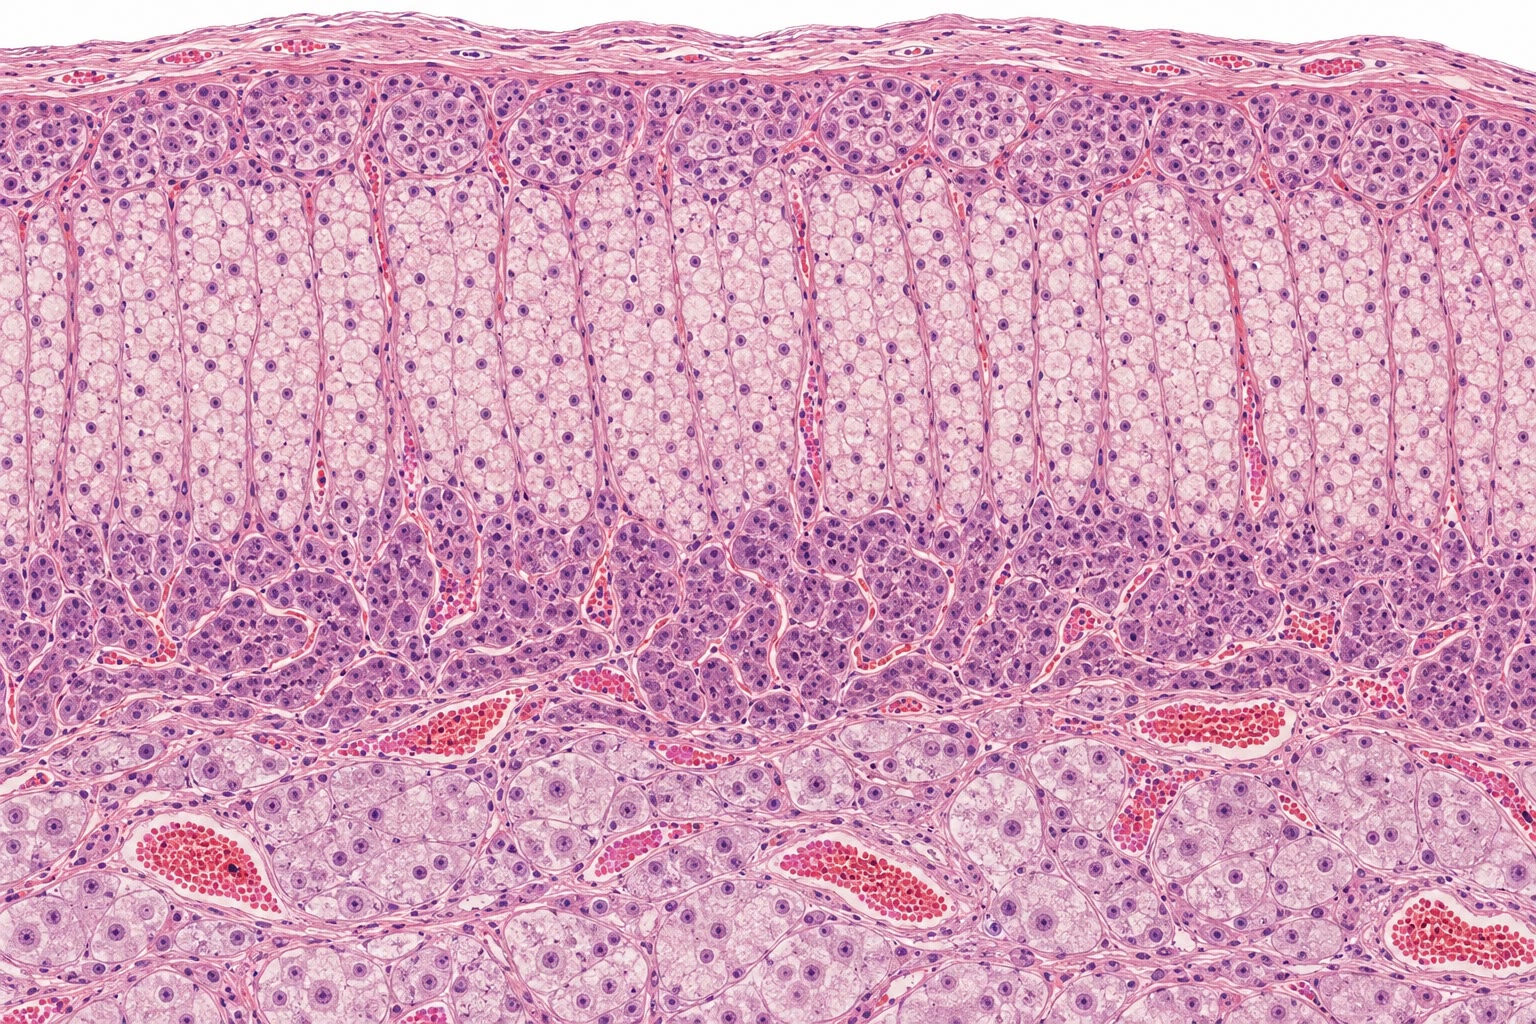
\includegraphics[width=0.5\linewidth]{images/book5/ai/b5-21-adrenal-section.jpg}\hspace{0.04\linewidth}
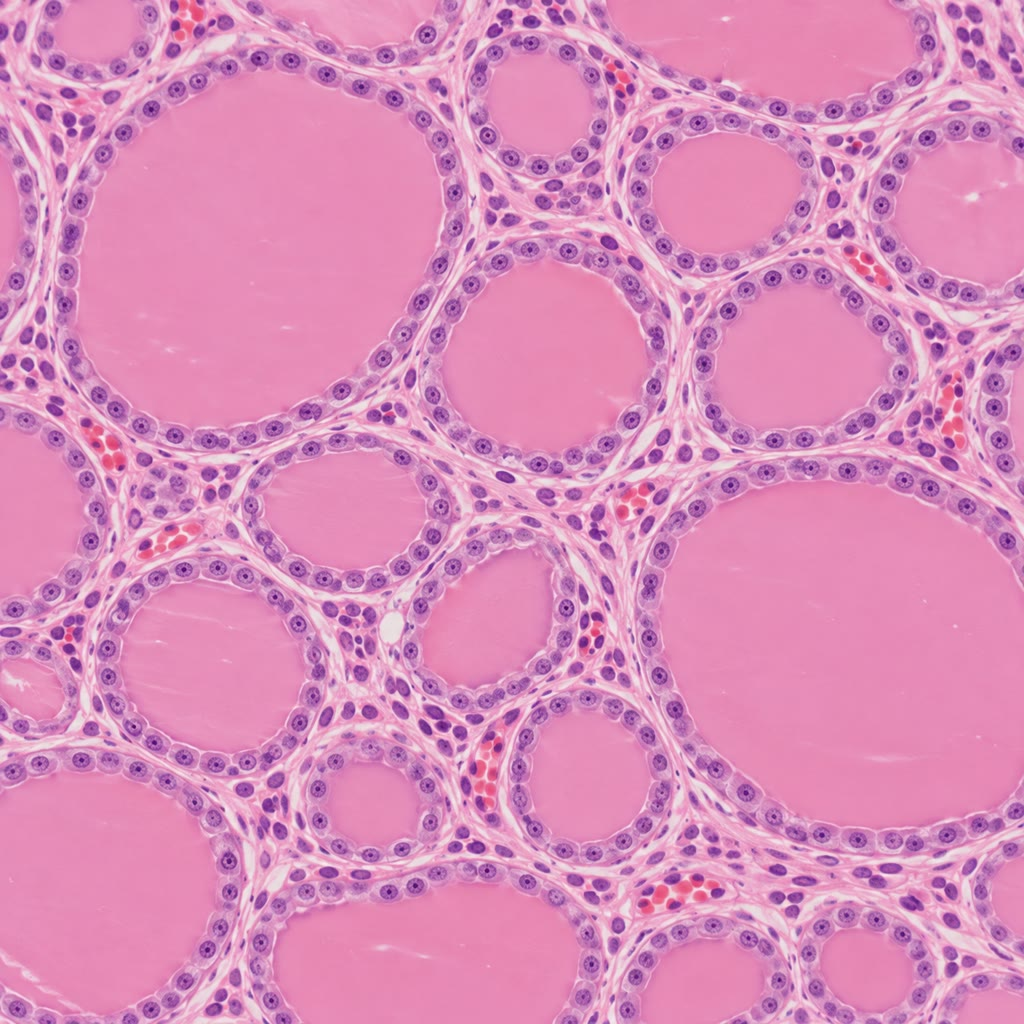
\includegraphics[width=0.36\linewidth]{images/book5/ai/b5-21-thyroid-follicles.jpg}

{\small À gauche~: la glande surrénale en coupe --- le cortex en ses
trois zones (l'\omterm{def:b3:renal-osmoregulation:controls}{aldostérone} la plus externe, le cortisol dans la large
zone moyenne, les androgènes la plus interne) autour d'une médullaire de
cellules chromaffines sécrétant l'adrénaline, qui est par son origine un
\omterm{def:b3:nervous-systems:comparative}{ganglion} sympathique. À droite~: des follicules thyroïdiens, chacun une
sphère de cellules autour d'une réserve de colloïde qui tient des mois
d'\omterm{def:b3:endocrinology:hormone}{hormone} liée à la thyroglobuline.}
\end{omfigure}

\section{Le glucose~: la boucle la plus serrée}

\begin{definition}[L'insuline et le glucagon]\label{def:b3:endocrinology:glucose}
\index{insuline}\index{glucagon}\index{îlot de Langerhans}\index{GLUT4}\index{diabète sucré}
Le sang contient environ \qty{5}{g} de glucose, à \qty{5}{mmol/L}
(\qty{90}{mg/dL}), et le cerveau en brûle \qty{120}{g} par jour et ne
peut rien brûler d'autre~; un repas en délivre \qty{75}{g} en une heure.
Les \emph{îlots de Langerhans}, un million d'amas de quelques milliers
de cellules dispersés dans le pancréas, tiennent la boucle. Les cellules
$\beta$ sentent le glucose en le métabolisant~: plus de glucose, plus
d'ATP, fermeture d'un canal potassique sensible à l'ATP,
dépolarisation, entrée de calcium et exocytose de l'\emph{insuline},
\omterm{def:b3:endocrinology:hormone}{hormone peptidique} découpée dans un précurseur unique. L'insuline dit au
muscle et au tissu adipeux d'amener le transporteur \emph{GLUT4} à leur
surface et de capter le glucose, au foie de stocker le glucose en
glycogène et de cesser d'en fabriquer, et au tissu adipeux de cesser de
libérer des acides gras~: c'est l'\omterm{def:b3:endocrinology:hormone}{hormone} de l'état nourri, la seule qui
abaisse la glycémie. Les cellules $\alpha$ libèrent le \emph{glucagon}
quand le glucose baisse~: le foie dégrade le glycogène et fabrique du
glucose neuf à partir d'acides aminés et de lactate. L'adrénaline, le
cortisol et l'\omterm{def:b3:endocrinology:hormone}{hormone} de croissance élèvent aussi le glucose, et la
redondance n'est pas symétrique~: un corps peut se défendre d'une baisse
par quatre voies et d'une hausse par une seule. Le \emph{diabète sucré}
est la défaillance de cette seule voie~: le type 1, destruction
auto-immune des cellules $\beta$, réclame de l'insuline dès le premier
jour~; le type 2, neuf cas sur dix, commence par une résistance des
tissus à l'insuline, à laquelle on répond des années durant par plus
d'insuline, jusqu'à ce que les cellules $\beta$ ne suivent plus et que
le glucose monte.
\end{definition}

\begin{theorem}[La boucle insuline--glucose]\label{thm:b3:endocrinology:loop}
\index{gain de boucle}\index{point de consigne}\index{oscillation amortie}
Notons $g$ et $i$ les écarts du glucose et de l'\omterm{def:b3:endocrinology:glucose}{insuline} plasmatiques à
leurs valeurs à jeun. Le glucose est éliminé à un rythme proportionnel à
son propre excès (l'efficacité du glucose $a$) et à l'excès d'\omterm{def:b3:endocrinology:glucose}{insuline}
(la sensibilité $s$)~; l'\omterm{def:b3:endocrinology:glucose}{insuline} est sécrétée proportionnellement à
l'excès de glucose ($\beta$) et éliminée au taux $\gamma$~; une charge
$u$ entre~:
\[
\dot g = -a\,g - s\,i + u, \qquad \dot i = \beta\,g - \gamma\,i .
\]
Sous une charge constante $u$ le glucose se fixe à
\[
g^{*} = \frac{u}{a}\cdot\frac{1}{1 + L}, \qquad L = \frac{s\beta}{a\gamma},
\]
de sorte que le rétrocontrôle divise par $1 + L$ la perturbation que
subirait un corps non régulé~: le \emph{\omterm{thm:b3:endocrinology:loop}{gain de boucle}} plus un. Après
un bolus le retour est gouverné par les valeurs propres
$\lambda = -\tfrac{a + \gamma}{2} \pm \sqrt{\tfrac{(a+\gamma)^{2}}{4} - (a\gamma + s\beta)}$~:
monotone si $s\beta < (a - \gamma)^{2}/4$, et sinon une \omterm{thm:b3:endocrinology:loop}{oscillation
amortie} de pulsation $\omega = \sqrt{a\gamma + s\beta -
(a+\gamma)^{2}/4}$ décroissant comme $\mathrm{e}^{-(a+\gamma)t/2}$ --- le
glucose passe sous sa valeur à jeun avant de se poser, ce qui est la
petite hypoglycémie deux ou trois heures après un repas sucré. La
résistance à l'\omterm{def:b3:endocrinology:glucose}{insuline} abaisse $s$~: l'état stationnaire à jeun sous la
production hépatique propre du corps monte, et la boucle compense par un
$i^{*}$ plus haut jusqu'à ce que le $\beta$ des cellules $\beta$ baisse à
son tour, et alors la compensation échoue.
\end{theorem}
\begin{proof}
État stationnaire~: $\dot i = 0$ donne $i^{*} = \beta g^{*}/\gamma$~; en
le portant dans $\dot g = 0$~: $a g^{*} + s\beta g^{*}/\gamma = u$, d'où
$g^{*} =
u/(a + s\beta/\gamma) = (u/a)/(1 + L)$. Dynamique~: la matrice du
système est
$\begin{pmatrix} -a & -s\\ \beta & -\gamma\end{pmatrix}$, de trace
$-(a+\gamma)$ et de déterminant $a\gamma + s\beta$~; son équation
caractéristique $\lambda^{2} + (a+\gamma)\lambda + (a\gamma + s\beta) = 0$
a les racines annoncées. Toutes deux ont une partie réelle négative,
donc l'état à jeun est stable~; les racines sont complexes quand le
discriminant $(a+\gamma)^{2}
- 4(a\gamma + s\beta) = (a-\gamma)^{2} - 4s\beta$ est négatif, la
condition donnée, et alors $g(t) = \mathrm{e}^{-(a+\gamma)t/2}(A\cos\omega t
+ B\sin\omega t)$, qui traverse zéro. La résistance~: avec $u$ la
production basale du foie et $s$ réduit, $L$ baisse et $g^{*}$ monte pour
le même $u$~; $i^{*} = \beta g^{*}/\gamma$ monte avec lui
(l'hyperinsulinémie)~; si $\beta$ baisse ensuite, $L$ baisse encore et
$g^{*}$ grimpe vers $u/a$.
\end{proof}

\begin{omfigure}
\begin{tikzpicture}
\begin{axis}[
  width=0.58\linewidth, height=5.6cm,
  axis x line=bottom, axis y line=left,
  xmin=0, xmax=180, ymin=40, ymax=200,
  xlabel={minutes après un bolus de glucose}, ylabel={glucose plasmatique (mg/dL)},
  xlabel style={font=\small, at={(axis description cs:0.5,-0.12)}, anchor=north}, ylabel style={font=\small},
  tick label style={font=\small}, xtick={0,30,60,90,120,150,180}, ytick={60,90,120,150,180},
  clip=false,
]
\addplot[very thick, omDef, smooth] coordinates {(0,190) (6,165) (12,131) (18,102) (24,84) (30,77) (36,78) (42,82) (48,86) (54,89) (60,91) (66,92) (72,91) (78,91) (84,90) (90,90) (96,90) (102,90) (108,90) (114,90) (120,90) (126,90) (132,90) (138,90) (144,90) (150,90) (156,90) (162,90) (168,90) (174,90) (180,90)};
\draw[dashed, gray] (axis cs:0,90) -- (axis cs:180,90);
\node[font=\scriptsize, gray, anchor=south east] at (axis cs:180,91) {niveau à jeun};
\node[font=\scriptsize, omDef, anchor=west, align=left] at (axis cs:75,150) {modèle~: $a = \qty{0.02}{min^{-1}}$, $\gamma = \qty{0.1}{min^{-1}}$,\\$s\beta = \qty{0.01}{min^{-2}}$, gain de boucle $L = 5$~;\\creux à \qty{32}{min}, période \qty{68}{min}};
\node[font=\scriptsize, omThm, anchor=north] at (axis cs:24,70) {creux};
\end{axis}
\begin{axis}[
  at={(0.6\linewidth,0)}, anchor=south west,
  width=0.33\linewidth, height=5.6cm,
  axis x line=bottom, axis y line=left,
  xmin=0, xmax=180, ymin=0, ymax=40,
  xlabel={minutes}, ylabel={insuline (mU/L)},
  xlabel style={font=\small, at={(axis description cs:0.5,-0.12)}, anchor=north}, ylabel style={font=\small},
  tick label style={font=\small}, xtick={0,60,120,180}, ytick={0,10,20,30,40},
]
\addplot[very thick, omProp, smooth] coordinates {(0,10.0) (6,30.0) (12,33.7) (18,28.5) (24,20.4) (30,13.4) (36,8.9) (42,7.1) (48,7.1) (54,7.9) (60,9.0) (66,9.8) (72,10.2) (78,10.4) (84,10.4) (90,10.2) (96,10.1) (102,10.0) (108,10.0) (114,9.9) (120,10.0) (126,10.0) (132,10.0) (138,10.0) (144,10.0) (150,10.0) (156,10.0) (162,10.0) (168,10.0) (174,10.0) (180,10.0)};
\draw[dashed, gray] (axis cs:0,10) -- (axis cs:180,10);
\end{axis}
\end{tikzpicture}

{\small La boucle linéaire après un bolus qui élève le glucose de
\qty{100}{mg/dL}. L'\omterm{def:b3:endocrinology:glucose}{insuline} culmine en moins de dix minutes et le
glucose est revenu à sa base en vingt, puis passe dessous~; un
rétrocontrôle fort qui agit par une \omterm{def:b3:endocrinology:hormone}{hormone} ayant son propre temps
d'élimination revient en \omterm{thm:b3:endocrinology:loop}{oscillation amortie} plutôt qu'en simple
décroissance.}
\end{omfigure}

\begin{proof}[Faits expérimentaux]
Von Mering et Minkowski (1889) retirèrent le pancréas d'un chien et
produisirent un diabète --- les mouches attroupées sur son urine
trahirent le sucre~; ligaturer les canaux, ce qui détruisait le tissu
digestif mais épargnait les îlots, ne le fit pas. Banting et Best
(1921), avec la purification de Collip, extrairent le principe des îlots
et abaissèrent la glycémie d'un chien diabétique, puis celle de Leonard
Thompson (janvier 1922). Sanger séquença l'\omterm{def:b3:endocrinology:glucose}{insuline} (1955), première
séquence protéique~; Yalow et Berson la mesurèrent dans le sang (1959)
et trouvèrent que les diabétiques d'apparition tardive en avaient
d'abord plus que les gens sains --- une résistance, non une carence. Les
bactéries de Genentech firent de l'\omterm{def:b3:endocrinology:glucose}{insuline} humaine en 1978, premier
médicament recombinant.
\end{proof}

\begin{omfigure}
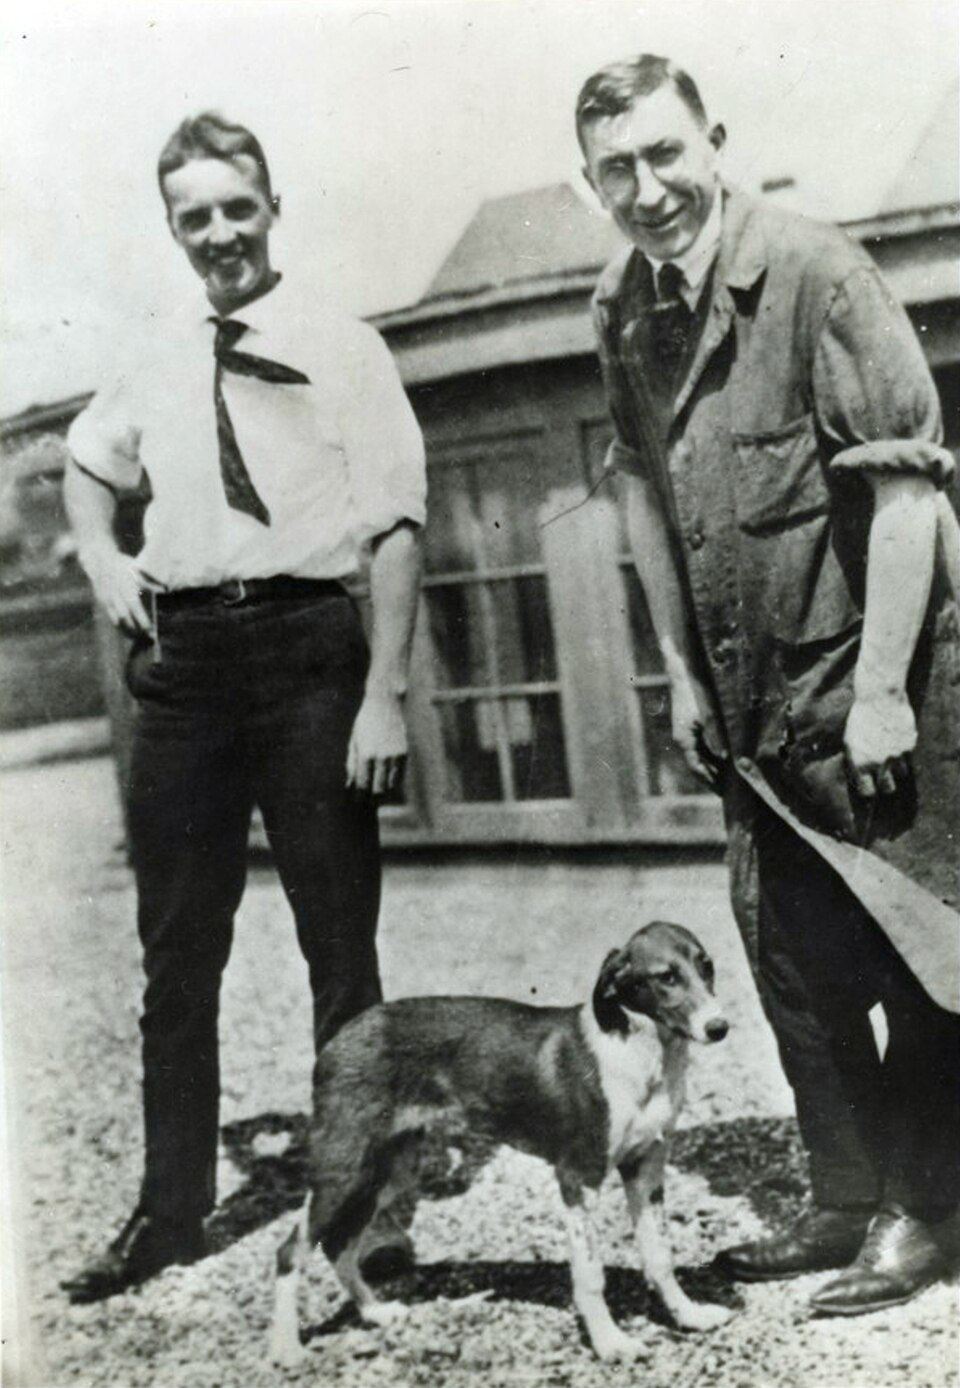
\includegraphics[width=0.42\linewidth]{images/book5/banting-best.jpg}\hspace{0.04\linewidth}
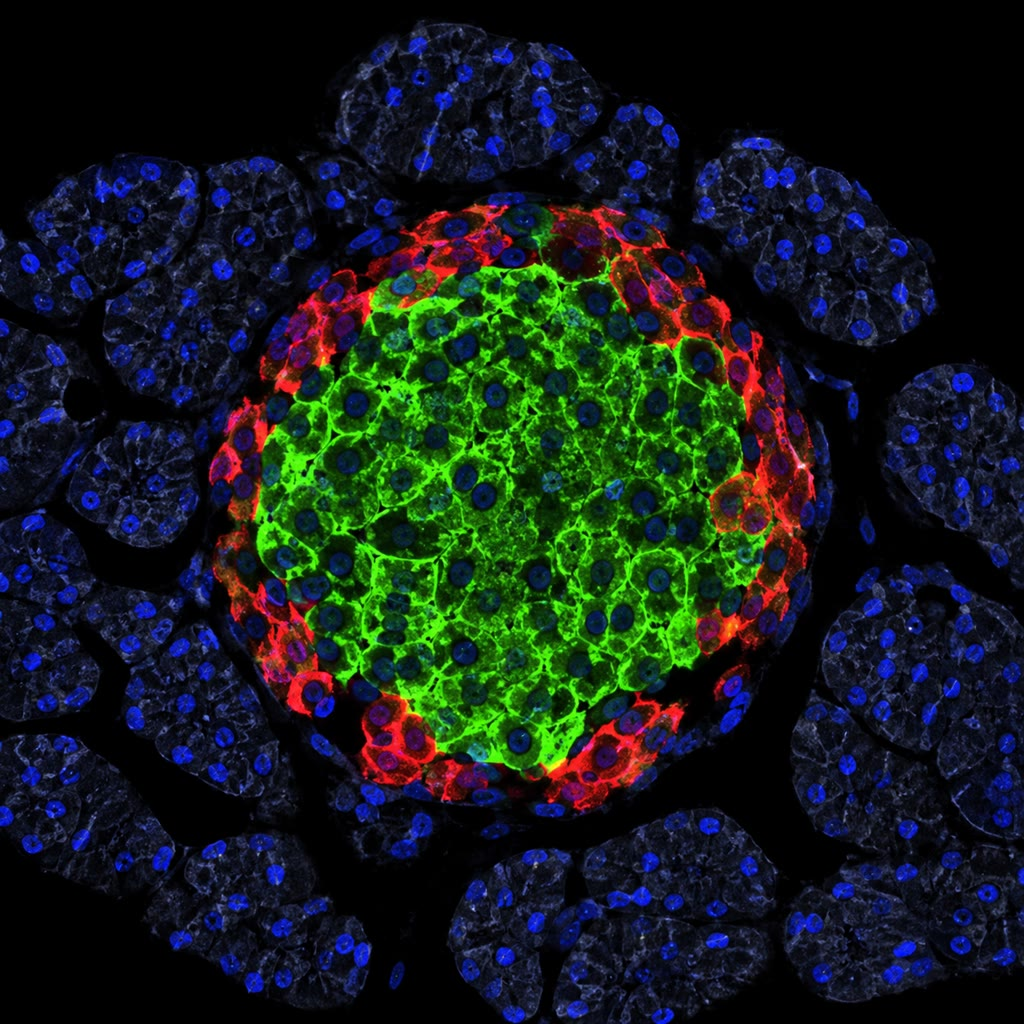
\includegraphics[width=0.42\linewidth]{images/book5/ai/b5-21-pancreatic-islet.jpg}

{\small À gauche~: Frederick Banting et Charles Best sur le toit du
bâtiment de médecine à Toronto, vers 1924, avec l'un des chiens des
expériences sur l'\omterm{def:b3:endocrinology:glucose}{insuline} (photographie dans le domaine public). À
droite~: un \omterm{def:b3:endocrinology:glucose}{îlot de Langerhans}, les cellules $\beta$ productrices
d'\omterm{def:b3:endocrinology:glucose}{insuline} au cœur, les cellules $\alpha$ à \omterm{def:b3:endocrinology:glucose}{glucagon} au pourtour, dans
une mer d'acini exocrines.}
\end{omfigure}

\begin{method}[Lire la boucle du glucose chez un patient]\label{met:b3:endocrinology:ogtt}
\index{test d'hyperglycémie provoquée}\index{HbA1c}
(1) La glycémie à jeun~: normale au-dessous de \qty{5.6}{mmol/L},
diabète à \qty{7.0}{mmol/L} ou plus à deux reprises. (2)
L'hyperglycémie provoquée par voie orale~: \qty{75}{g} de glucose bus~;
la glycémie à deux heures est normale au-dessous de \qty{7.8}{mmol/L},
diabétique à \qty{11.1}{mmol/L} ou plus --- la valeur à deux heures lit
le gain de la boucle, celle à jeun son \omterm{thm:b3:endocrinology:loop}{point de consigne}. (3)
L'hémoglobine glyquée, l'\emph{HbA1c}~: le glucose s'attache
irréversiblement à l'hémoglobine à un rythme proportionnel à sa
concentration, et les globules rouges vivent 120 jours, de sorte que la
fraction glyquée intègre la glycémie moyenne des trois derniers mois
sans qu'il faille être à jeun --- normale au-dessous de \qty{5.7}{\%},
diabétique à partir de \qty{6.5}{\%}. (4) Pour séparer la résistance de
la carence, doser l'\omterm{def:b3:endocrinology:glucose}{insuline} (ou son sous-produit, le peptide~C) à
côté~: une \omterm{def:b3:endocrinology:glucose}{insuline} élevée avec un glucose élevé est une résistance~; un
peptide~C absent est un type~1.
\end{method}

\section{Le calcium, et l'horloge}

\begin{definition}[L'homéostasie du calcium]\label{def:b3:endocrinology:calcium}
\index{parathormone}\index{calcitriol}\index{vitamine D}\index{ostéoporose}
Le calcium ionisé du plasma est tenu à \qty{1.2}{mmol/L} à quelques pour
cent près, parce qu'il fixe l'excitabilité de tout nerf et de tout
muscle~: trop bas et ils déchargent spontanément (la tétanie), trop haut
et ils deviennent mous. Les quatre glandes parathyroïdes le sentent par
un récepteur de surface et sécrètent la \emph{parathormone} (PTH) le
long d'une sigmoïde inverse très raide~: la PTH mobilise le calcium de
l'os, fait au rein réabsorber le calcium et excréter le phosphate, et
active la \emph{vitamine~D} --- faite dans la peau par l'ultraviolet ou
mangée, hydroxylée dans le foie puis dans le rein en \emph{calcitriol}
--- qui fait absorber le calcium par l'intestin. L'os est le réservoir,
un kilogramme de calcium, remanié sans cesse par les ostéoclastes et les
ostéoblastes sous la PTH, le calcitriol, les œstrogènes et la charge.
La carence en vitamine~D donne le rachitisme chez l'enfant et des os
mous chez l'adulte~; la chute des œstrogènes à la ménopause fait pencher
le remaniement vers la résorption et donne l'\emph{ostéoporose}~; un
adénome parathyroïdien élève le calcium, dissout l'os et forme des
calculs rénaux --- «~des os, des pierres, des plaintes et des gémissements~».
\end{definition}

\begin{definition}[L'horloge circadienne]\label{def:b3:endocrinology:clock}
\index{horloge circadienne}\index{noyau suprachiasmatique}\index{gènes de l'horloge}\index{mélatonine}\index{zeitgeber}
Presque toute cellule porte une \emph{horloge circadienne}~: une boucle
de transcription et de traduction où les protéines CLOCK et BMAL1
allument les gènes \emph{Per} et \emph{Cry}, dont les protéines
s'accumulent, entrent dans le noyau après un retard de quelques heures
et répriment leur propre transcription, puis sont dégradées, ce qui lève
la répression --- un cycle en vingt-quatre heures environ, fixé par les
vitesses du retard et de la dégradation. Les horloges du corps sont
synchronisées par une horloge maîtresse de vingt mille neurones du
\emph{noyau suprachiasmatique} de l'\omterm{def:b3:endocrinology:axes}{hypothalamus}, elle-même mise à
l'heure par la lumière grâce à une classe dédiée de \omterm{def:b3:sensory-systems:retina}{cellules
ganglionnaires} de la \omterm{def:b3:sensory-systems:retina}{rétine} (qui contiennent de la mélanopsine, non les
pigments des \omterm{def:b3:sensory-systems:retina}{bâtonnets} ni des \omterm{def:b3:sensory-systems:retina}{cônes}), et qui signale la nuit au corps
par la \emph{mélatonine} de l'épiphyse, sécrétée dans l'obscurité seule.
L'horloge programme le cortisol avant le réveil, la température
corporelle la plus basse à 4 heures du matin, l'\omterm{def:b3:endocrinology:hormone}{hormone} de croissance
dans le premier sommeil, une sensibilité à l'\omterm{def:b3:endocrinology:glucose}{insuline} plus haute le
matin~; la nourriture, l'exercice et la température sont des
\emph{zeitgebers} secondaires qui peuvent écarter les horloges
périphériques de l'horloge centrale, ce qui fait le malaise du
travailleur posté et du décalage horaire --- une horloge du foie à une
heure et un cerveau à une autre.
\end{definition}

\begin{proof}[Faits expérimentaux]
Konopka et Benzer (1971) criblèrent des mouches mutantes pour des
rythmes d'émergence altérés et trouvèrent trois allèles d'un même gène,
\emph{period}~: un jour court (19 h), un jour long (29 h), et aucun
rythme du tout --- une horloge à période génétique. Hardin, Hall et
Rosbash (1990) trouvèrent que l'ARNm et la protéine de \emph{period}
oscillent avec un décalage entre eux, et que la protéine réprime son
propre gène~: la boucle. Ralph et Menaker (1990) greffèrent le \omterm{def:b3:endocrinology:clock}{noyau
suprachiasmatique} d'un hamster mutant à rythme de 20 heures dans un
hamster normal dont le propre noyau avait été détruit~: le receveur
tourna sur 20 heures --- la période appartenait au tissu greffé. Chez
des humains tenus dans un bunker sans repère temporel le rythme courait
librement à un peu plus de 24 heures~; une lumière vive le soir le
retardait, le matin l'avançait.
\end{proof}

\begin{omfigure}
\begin{tikzpicture}[every node/.style={font=\scriptsize}, >=stealth]
  \node[draw, thick, rounded corners, fill=omDef!20, align=center] (cb) at (0,1.6) {activateurs\\CLOCK--BMAL1};
  \node[draw, thick, rounded corners, fill=omProp!25, align=center] (pc) at (3.6,1.6) {\emph{Per}, \emph{Cry}\\transcrits};
  \node[draw, thick, rounded corners, fill=omThm!20, align=center] (pr) at (3.6,-0.4) {les protéines PER, CRY\\s'accumulent, se dimérisent};
  \node[draw, thick, rounded corners, fill=omMeth!25, align=center] (nu) at (0,-0.4) {entrent dans le noyau\\après des heures};
  \draw[->, thick] (cb) -- (pc) node[midway, above, font=\tiny] {activent};
  \draw[->, thick] (pc) -- (pr) node[midway, right, font=\tiny] {traduction, retard};
  \draw[->, thick] (pr) -- (nu);
  \draw[-|, thick, omThm] (nu) -- (cb) node[midway, left, font=\tiny, omThm, align=right] {répriment\\leurs propres\\activateurs};
  \draw[->, thick, gray] (nu.south) -- ++(0,-0.5) node[below, font=\tiny, gray] {dégradées~: la répression se lève, cycle $\approx$ \qty{24}{h}};
  % right: daily profile
  \begin{scope}[shift={(7.2,-1.6)}]
    \draw[->] (0,0) -- (5.6,0) node[right, font=\tiny] {heure};
    \draw[->] (0,0) -- (0,3.4);
    \foreach \x/\l in {0/0, 1.4/6, 2.8/12, 4.2/18, 5.6/24} { \draw (\x,0) -- (\x,-0.08) node[below, font=\tiny] {\l}; }
    \fill[gray!25] (0,0) rectangle (1.4,3.4); \fill[gray!25] (5.1,0) rectangle (5.6,3.4);
    \node[font=\tiny, gray!60!black] at (0.7,3.2) {nuit};
    \draw[very thick, omMeth!70!black, domain=0:5.6, samples=60, smooth, variable=\x] plot (\x, {1.6 + 1.2*cos(deg(2*3.1416*(\x-1.9)/5.6))});
    \node[font=\tiny, omMeth!70!black] at (3.1,3.1) {cortisol~: pic à 8 h};
    \draw[very thick, omDef, domain=0:5.6, samples=60, smooth, variable=\x] plot (\x, {0.9 + 0.7*cos(deg(2*3.1416*(\x-0.7)/5.6))});
    \node[font=\tiny, omDef] at (2.7,0.18) {mélatonine~: la nuit seulement};
  \end{scope}
\end{tikzpicture}

{\small À gauche~: le cœur de l'horloge moléculaire, une boucle de
\omterm{def:b3:endocrinology:axes}{rétrocontrôle négatif} avec un retard de quelques heures, ce dont une
boucle a besoin pour osciller plutôt que se poser. À droite~: deux
\omterm{def:b3:endocrinology:hormone}{hormones} qu'elle programme --- le cortisol qui monte avant l'aube pour
préparer la journée, la \omterm{def:b3:endocrinology:clock}{mélatonine} qui marque la nuit.}
\end{omfigure}

\begin{remark}[L'homéostasie comme commande]\label{rem:b3:endocrinology:control}
Toute boucle de ce chapitre a les mêmes pièces~: un capteur (le
métabolisme de la cellule $\beta$, le récepteur du calcium de la
parathyroïde, le récepteur des \omterm{prop:b3:endocrinology:thyroid}{hormones thyroïdiennes} de l'\omterm{def:b3:endocrinology:axes}{hypophyse}),
un régulateur qui compare à un \omterm{thm:b3:endocrinology:loop}{point de consigne}, une \omterm{def:b3:endocrinology:hormone}{hormone} effectrice
avec sa propre demi-vie, et un rétrocontrôle qui réduit l'erreur d'un
facteur $1 + L$ mais jamais à zéro. Ce qui diffère est le tempo ---
quelques secondes pour l'adrénaline, une heure pour l'\omterm{def:b3:endocrinology:glucose}{insuline}, des
jours pour la thyroxine, une vie pour l'os --- et le prix du compromis~:
une boucle rapide à effecteur retardé oscille, une boucle lente laisse
une perturbation s'installer. La clinique voit les boucles du dehors,
par les couples que le rétrocontrôle associe~: une TSH élevée avec une
T$_{4}$ basse est une glande défaillante, une TSH élevée avec une
T$_{4}$ élevée une \omterm{def:b3:endocrinology:axes}{hypophyse} défaillante~; une \omterm{def:b3:endocrinology:glucose}{insuline} élevée avec un
glucose élevé est une résistance, une \omterm{def:b3:endocrinology:glucose}{insuline} basse avec un glucose
élevé une destruction. Pour lire le niveau d'une \omterm{def:b3:endocrinology:hormone}{hormone} il faut
toujours demander ce que faisait celui qui la commande.
\end{remark}

\section{Exercices}

\begin{exercise}[$\star$]\label{exo:b3:endocrinology:1}
Classer l'\omterm{def:b3:endocrinology:glucose}{insuline}, le cortisol, l'adrénaline, la thyroxine et la
vasopressine par chimie, localisation du récepteur, rapidité d'action et
demi-vie.
\end{exercise}

\begin{exercise}[$\star$]\label{exo:b3:endocrinology:2}
Dessiner l'axe thyroïdien avec son rétrocontrôle et prévoir la TSH et la
T$_{4}$ dans~: une thyroïde détruite~; une \omterm{def:b3:cancer-biology:hallmarks}{tumeur} hypophysaire sécrétant
la TSH~; un patient qui prend trop de thyroxine~; une carence en iode.
\end{exercise}

\begin{exercise}[$\star$]\label{exo:b3:endocrinology:3}
Pourquoi un corps a-t-il quatre \omterm{def:b3:endocrinology:hormone}{hormones} qui élèvent la glycémie et une
seule qui l'abaisse~? Que cela prédit-il des dangers relatifs d'un excès
et d'un défaut d'\omterm{def:b3:endocrinology:glucose}{insuline}~?
\end{exercise}

\begin{exercise}[$\star$]\label{exo:b3:endocrinology:4}
Qu'est-ce qu'un \omterm{def:b3:endocrinology:clock}{zeitgeber}~? En donner trois, dire lequel l'horloge
maîtresse emploie, et expliquer ce qui arrive à un voyageur qui traverse
huit fuseaux horaires.
\end{exercise}

\begin{exercise}[$\star\star$]\label{exo:b3:endocrinology:5}
Une cellule a \num{20000} récepteurs de $K_{d} = \qty{1}{nM}$ et répond
au maximum quand \num{500} sont occupés. Trouver la CE$_{50}$. Après une
semaine d'\omterm{def:b3:endocrinology:hormone}{hormone} élevée la cellule n'a plus que \num{2000} récepteurs~:
nouvelle CE$_{50}$~? Interpréter pour la résistance à l'\omterm{def:b3:endocrinology:glucose}{insuline}.
\end{exercise}

\begin{exercise}[$\star\star$]\label{exo:b3:endocrinology:6}
Avec $\kappa = \qty{0.46}{L/pmol}$ et une TSH normale de \qty{1.5}{mU/L}
pour une T$_{4}$ libre de \qty{15}{pmol/L}, calculer la TSH quand
T$_{4}$ vaut $13$, $11$, $9$ et \qty{25}{pmol/L}. Pour lesquelles de ces
valeurs T$_{4}$ serait-elle encore dans une plage de référence de
\qtyrange{10}{20}{pmol/L} alors que la TSH est hors de
\qtyrange{0.4}{4}{mU/L}~?
\end{exercise}

\begin{exercise}[$\star\star$]\label{exo:b3:endocrinology:7}
Dans la boucle du \cref{thm:b3:endocrinology:loop} avec $a = \qty{0.02}{min^{-1}}$,
$\gamma = \qty{0.1}{min^{-1}}$, $\beta = \qty{0.05}{mU\,L^{-1}\,min^{-1}}$
par mg/dL et $s = \qty{0.2}{mg\,dL^{-1}\,min^{-1}}$ par mU/L, calculer
le \omterm{thm:b3:endocrinology:loop}{gain de boucle}, l'excès de glucose stationnaire sous une charge
constante de \qty{2}{mg/dL/min}, le même sans rétrocontrôle, et l'excès
d'\omterm{def:b3:endocrinology:glucose}{insuline} stationnaire.
\end{exercise}

\begin{exercise}[$\star\star$]\label{exo:b3:endocrinology:8}
Mêmes paramètres~: le retour après un bolus est-il oscillatoire~?
Calculer la période et le temps pour que l'amplitude baisse d'un facteur
$\mathrm{e}$. Diviser maintenant $s$ par deux (résistance à l'\omterm{def:b3:endocrinology:glucose}{insuline})~:
recalculer les deux et le nouveau \omterm{thm:b3:endocrinology:loop}{gain de boucle}.
\end{exercise}

\begin{exercise}[$\star\star$]\label{exo:b3:endocrinology:9}
La demi-vie du cortisol est de \qty{80}{min}. Un patient sous
\qty{40}{mg} de prednisolone par jour depuis un an s'arrête brutalement.
Expliquer, étage par étage, pourquoi il peut s'effondrer sur une
infection bénigne trois jours plus tard, et ce que montrerait l'axe si
on le mesurait (ACTH, cortisol, réponse à l'ACTH injectée).
\end{exercise}

\begin{exercise}[$\star\star\star$]\label{exo:b3:endocrinology:10}
Montrer qu'un \omterm{def:b3:endocrinology:axes}{rétrocontrôle négatif} à une variable $\dot x = f(x)$ avec
$f' < 0$ ne peut osciller, alors que la boucle à deux variables du
théorème le peut, et expliquer avec des mots pourquoi l'horloge a besoin
d'un retard de quelques heures entre la transcription et la répression
pour produire une période de 24 heures. Qu'arriverait-il à la période si
PER était dégradée deux fois plus vite~?
\end{exercise}

\begin{exercise}[$\star\star\star$]\label{exo:b3:endocrinology:11}
La \omterm{def:b3:endocrinology:calcium}{parathormone} suit $\text{PTH} = P_{\max}/(1 +
\mathrm{e}^{k(\text{Ca} - \text{Ca}_{0})})$ avec $\text{Ca}_{0} =
\qty{1.2}{mmol/L}$ et $k = \qty{20}{L/mmol}$. Calculer la PTH en
fraction du maximum pour Ca $= 1.10$, $1.15$, $1.20$, $1.25$ et \qty{1.30}{mmol/L},
la pente au \omterm{thm:b3:endocrinology:loop}{point de consigne}, et expliquer pourquoi une telle raideur
est souhaitable pour le calcium mais serait dangereuse pour le glucose.
\end{exercise}

\begin{exercise}[$\star\star\star$]\label{exo:b3:endocrinology:12}
Le glucose s'attache à l'hémoglobine au rythme $k\,G$ par unité de
temps, avec $k$ tel qu'une glycémie moyenne de \qty{5.5}{mmol/L} donne
\qty{5}{\%} de glycation sur les 120 jours de vie d'un globule rouge.
Établir l'HbA1c en fonction de la glycémie moyenne, la valeur à
\qty{10}{mmol/L}, et expliquer pourquoi un patient atteint d'anémie
hémolytique (globules vivant 60 jours) a une HbA1c trompeusement basse.
\end{exercise}

\section{Problème~: le sucre dans le sang}

\begin{problem}[{Problème du week-end --- une hyperglycémie provoquée
lue à travers la boucle linéaire insuline--glucose~: la répartition d'une
dose de \qty{75}{g}, le \omterm{thm:b3:endocrinology:loop}{gain de boucle} et le retour amorti, ce que la
résistance et la défaillance des cellules $\beta$ font au \omterm{thm:b3:endocrinology:loop}{point de
consigne} à jeun, un diagnostic tiré des nombres, et l'axe thyroïdien à
côté, pour finir sur le \omterm{thm:b3:endocrinology:loop}{gain de boucle}, le temps de retour et la
glycémie à jeun de la boucle défaillante}]
\label{pb:b3:endocrinology:1}
Données~: un adulte sain, volume de distribution du glucose \qty{15}{L},
glycémie à jeun \qty{90}{mg/dL} (\qty{5}{mmol/L}), \omterm{def:b3:endocrinology:glucose}{insuline} à jeun
\qty{10}{mU/L}. Paramètres de la boucle~: $a = \qty{0.02}{min^{-1}}$, $\gamma =
\qty{0.1}{min^{-1}}$, $\beta = 0.05$ (mU/L par min et par mg/dL), $s = 0.2$
(mg/dL par min et par mU/L). Production hépatique basale de glucose $u_{0} =
\qty{2}{mg/dL/min}$ (déjà compensée à l'état à jeun par l'élimination à
jeun). Une dose orale de \qty{75}{g} est absorbée en une heure.
Thyroïde~: $\text{TSH} = 1.5\,\mathrm{e}^{-0.46(T_{4} - 15)}$ mU/L. Masse
molaire du glucose \qty{180}{g/mol}.

\medskip
\noindent\textbf{Partie I --- La dose.}
\begin{enumerate}
  \item Exprimer la glycémie à jeun en mmol/L et vérifier la conversion
        depuis les mg/dL. Combien de grammes de glucose y a-t-il dans le
        volume de distribution à jeun~?
  \item Si les \qty{75}{g} entiers apparaissaient d'un coup dans
        \qty{15}{L}, de combien le glucose monterait-il (en mg/dL et en
        mmol/L)~? Pourquoi le pic réel, environ \qty{60}{mg/dL} au-dessus
        du jeûne, en est-il si loin~?
  \item Absorbée en \qty{60}{min}, la dose entre à quel rythme en mg/dL
        par minute~? Comparer à $u_{0}$.
  \item Sans aucune réponse insulinique ($s = 0$), le glucose suivrait $\dot
        g = -a g + u$. Excès stationnaire sous le rythme d'absorption, et
        constante de temps de l'approche. Où serait le glucose après une
        heure~?
  \item Avec la boucle, calculer $L$ et l'excès stationnaire sous le même
        rythme. Comparer à la question~4.
  \item Expliquer pourquoi le cerveau est protégé des deux côtés~: ce
        dont il a besoin, et ce que trop de glucose fait aux tissus au
        fil des ans.
\end{enumerate}

\medskip
\noindent\textbf{Partie II --- Le retour.}
\begin{enumerate}[resume]
  \item Écrire l'équation caractéristique de la boucle et calculer la
        trace, le déterminant et le discriminant.
  \item Calculer $\omega$ et la période de l'\omterm{thm:b3:endocrinology:loop}{oscillation amortie}, ainsi
        que le temps de décroissance $2/(a + \gamma)$.
  \item En partant d'un excès de \qty{100}{mg/dL} avec l'\omterm{def:b3:endocrinology:glucose}{insuline} à sa
        valeur à jeun, la solution est $g(t) = 100\,\mathrm{e}^{-0.06t}
        (\cos\omega t + c\sin\omega t)$. Trouver $c$ d'après $\dot g(0) = -a\cdot
        100$.
  \item Quand le glucose revient-il pour la première fois au jeûne (le
        premier zéro de $g$)~? Estimer le creux au premier minimum.
  \item L'\omterm{def:b3:endocrinology:glucose}{insuline}~: $i(t)$ a la même exponentielle et la même
        pulsation. Argumenter d'après $\dot i = \beta g - \gamma i$ que
        son pic vient après que le glucose a commencé à baisser et avant
        qu'il n'atteigne le jeûne.
  \item Pourquoi une vraie épreuve de tolérance, avec une absorption sur
        une heure plutôt qu'un bolus, montre-t-elle un pic à 30--60
        minutes et un retour à deux heures, et seulement un léger creux
        à trois~?
\end{enumerate}

\medskip
\noindent\textbf{Partie III --- Quand la boucle lâche.}
\begin{enumerate}[resume]
  \item La résistance à l'\omterm{def:b3:endocrinology:glucose}{insuline} divise $s$ par deux. Nouveau $L$~? Le
        $u_{0}$ du foie est maintenant compensé par un nouvel état
        stationnaire à jeun~: en prenant $g^{*} = (u_{0}/a)/(1
        + L)$ comme excès sur une base idéalisée non régulée, trouver de
        combien la glycémie à jeun monte par rapport à l'état sain
        (calculer les deux $g^{*}$ et soustraire).
  \item \omterm{def:b3:endocrinology:glucose}{Insuline} à jeun dans l'état résistant~: calculer $i^{*} = \beta
        g^{*}/\gamma$ pour les deux états et le rapport. Comment la
        clinique appelle-t-elle cela~?
  \item Les cellules $\beta$ défaillent à leur tour~: $\beta$ tombe aussi
        au cinquième. Nouveau $L$, nouvel excès à jeun. Convertir en
        mmol/L et comparer au seuil diabétique de \qty{7}{mmol/L}.
  \item Le retour est-il encore oscillatoire dans l'état de la
        question~15~? Calculer le discriminant et la constante de temps
        du mode le plus lent.
  \item Un patient a une glycémie à jeun de \qty{8}{mmol/L}, une
        \omterm{def:b3:endocrinology:glucose}{insuline} à jeun de \qty{30}{mU/L}, une valeur à deux heures de
        \qty{13}{mmol/L}. Diagnostiquer le type et le mécanisme d'après
        les couples.
  \item Un autre a une glycémie à jeun de \qty{15}{mmol/L}, un
        peptide~C indétectable, et a perdu \qty{8}{kg} en deux mois.
        Diagnostiquer, et expliquer l'amaigrissement par ce que font les
        tissus sans \omterm{def:b3:endocrinology:glucose}{insuline}.
  \item HbA1c~: si la glycémie moyenne du premier patient vaut
        \qty{9}{mmol/L}, et que \qty{5.5}{mmol/L} donne \qty{5}{\%},
        estimer son HbA1c en supposant la proportionnalité.
\end{enumerate}

\medskip
\noindent\textbf{Partie IV --- La glande d'à côté.}
\begin{enumerate}[resume]
  \item La T$_{4}$ libre vaut \qty{12}{pmol/L}. Calculer la TSH. La
        T$_{4}$ est-elle dans la plage \qtyrange{10}{20}{pmol/L}~? La TSH
        est-elle dans \qtyrange{0.4}{4}{mU/L}~? Comment appelle-t-on cet
        état~?
  \item T$_{4}$ vaut \qty{7}{pmol/L}~: TSH~? Un patient avec cette
        T$_{4}$ mais une TSH de \qty{0.3}{mU/L}~: où est la lésion~?
  \item La demi-vie de la thyroxine est de \qty{7}{d}. Un patient sous
        substitution oublie une semaine de comprimés. À quelle fraction
        le niveau tombe-t-il, et pourquoi la semaine manquée est-elle
        moins dangereuse qu'un jour manqué de substitution en cortisol~?
  \item La maladie de Basedow~: un \omterm{def:b3:adaptive-immunity:antibody}{anticorps} occupe le récepteur de la
        TSH. Prévoir T$_{4}$, TSH, et l'effet de la relation log-linéaire
        sur la TSH mesurée.
  \item Expliquer en un paragraphe pourquoi le niveau d'une \omterm{def:b3:endocrinology:hormone}{hormone} n'a
        pas de sens sans le niveau de celle qui la commande, en utilisant
        les quatre couples de la dernière remarque du chapitre.
  \item Résumer~: le gain de la boucle saine (question~5), la période et
        le temps de décroissance du retour (question~8), et la glycémie à
        jeun de la boucle défaillante (question~15).
\end{enumerate}
\end{problem}
